\documentclass[12pt]{article}
\usepackage[tmargin=1.5in]{geometry}
\usepackage{relsize}
\usepackage{babel}
\usepackage{listings}
\usepackage{amsmath}
\usepackage{amssymb}
\usepackage[table]{xcolor}
\usepackage[pdftex]{graphicx}
\usepackage{caption}
\usepackage{rotating}

\setlength{\parindent}{0cm}  % Indentation prohibited by default

\title{Aufgabenblatt 10: Schema Gauss-Seidel}
\author{Gruppe: CaesarBaurMueller}
\date{\today}

\begin{document}
\maketitle

\begin{sloppypar}

\section*{Abbruchkommunikation}
In unserem Schema für Gauss-Seidel, kann ein Prozess immer dann eine weitere Iteration durchführen, wenn sein Nachfolger maximal eine Iteration zurückliegt. Dies ist der Fall, da die jeweilige erste Zeile aus der selben Iteration zur Berechnung des eigenen Matrixteils benötigt wird.

Eine Visualisierung findet sich in der nachfolgenden Grafik.

\begin{sidewaysfigure}
    \centering
    \vspace*{3em}
    \hspace*{-1em}
    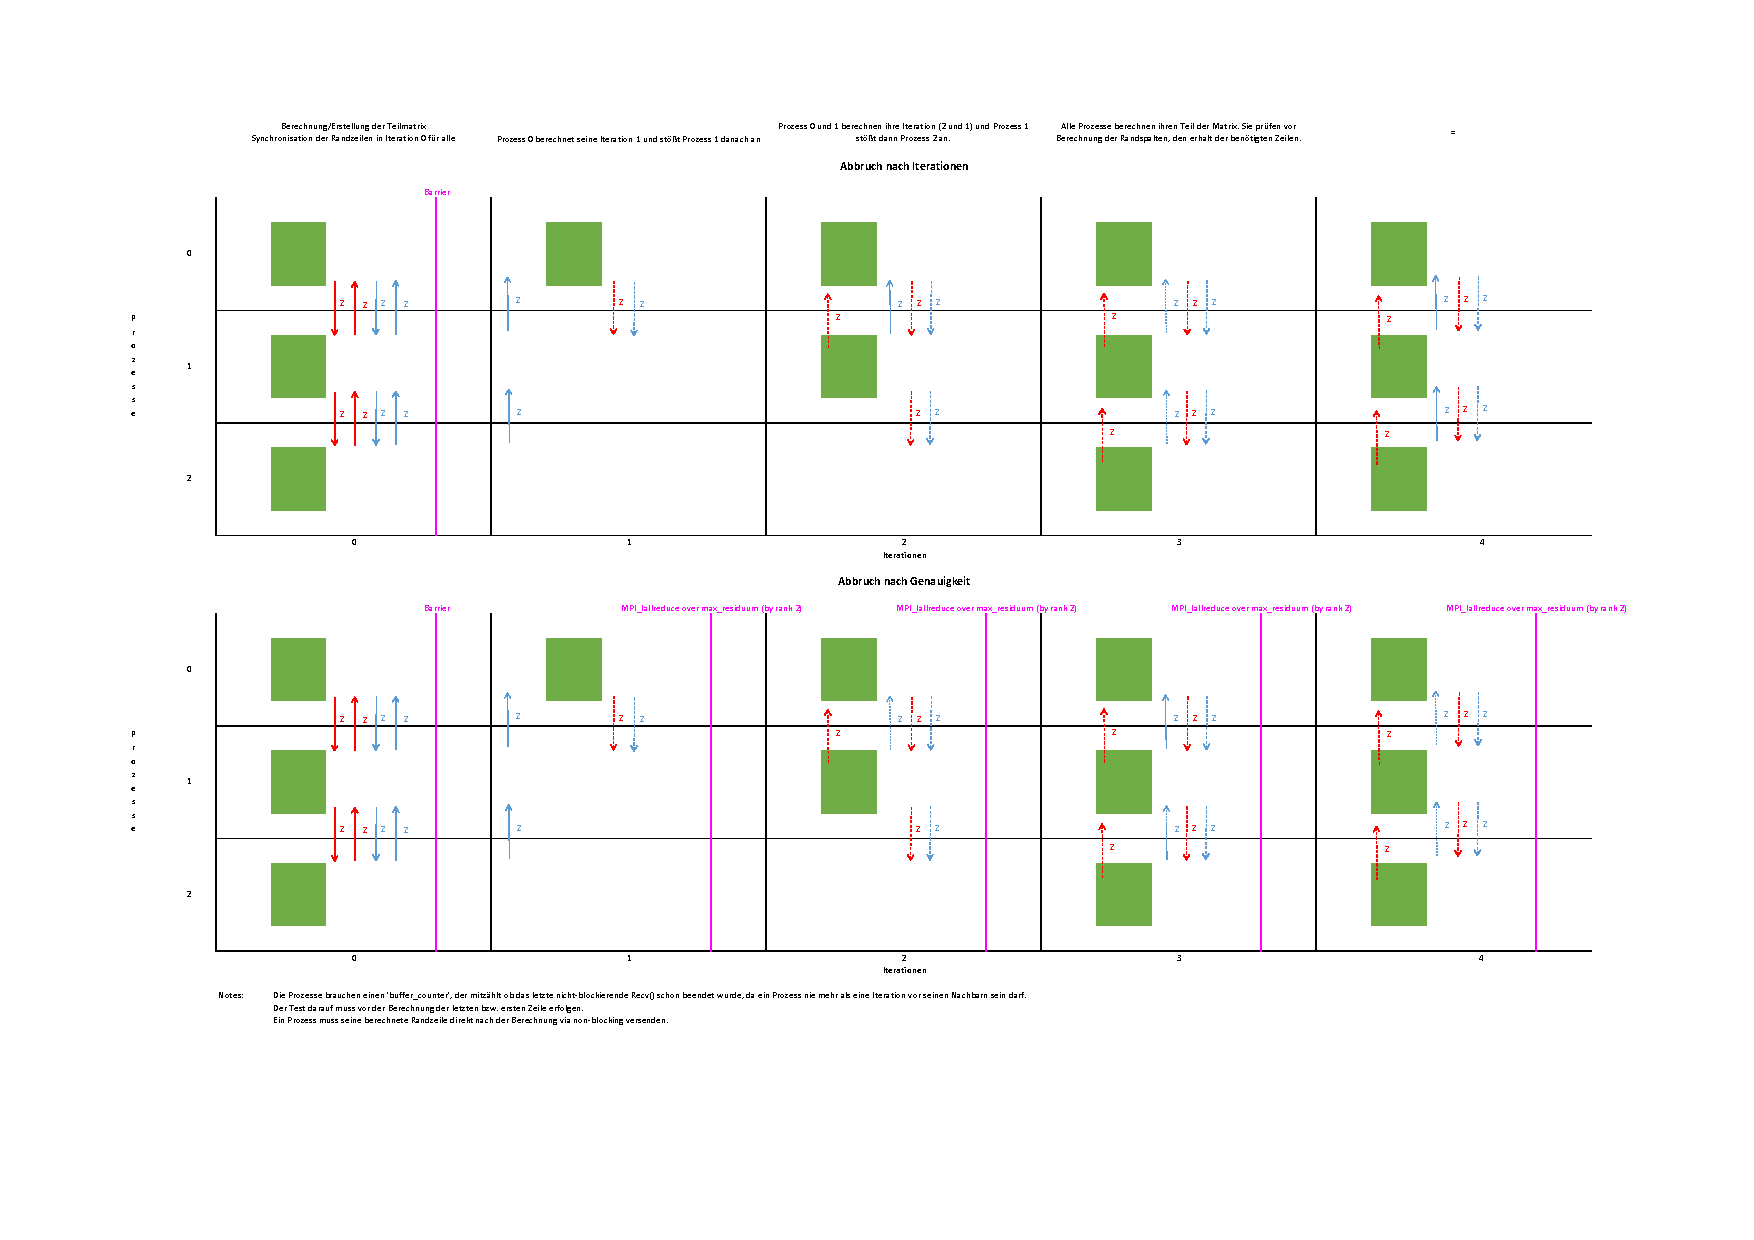
\includegraphics[width=1.1\textwidth]{res/Kommunikationsschema_gauss_seidel.pdf}
\end{sidewaysfigure}

\setcounter{section}{1}

\subsection{Abbruch nach Iterationen}
Der Abbruch nach Iterationen ist in unserem Programm vergleichsweise einfach. Jeder Prozess prüft für sich in jeder Iteration, ob er seine Endbedingung \verb|aktuelle_iteration == max_iteration| erfüllt hat. Ist dies der Fall, wird dieser Prozess abgebrochen. Die restlichen Prozesse laufen solange weiter, bis ihre jeweiligen Abbruchbedingungen jeweils erfüllt sind. Da jeder Prozess nur maximal eine Iteration von seinen Nachbarn entfernt sein kann, kommt es hier zu keinen Problemen, was die Kommunikation angeht.

\subsection{Abbruch nach Genauigkeit}
Die Abbruchbedingung lautet: \verb|max_residuum_of_all_procs < term_precision|.

\hspace*{2em}

Dies stellt uns jedoch vor ein Problem. Wir können nicht so wie bei dem Abbruch nach Iterationen jeden Prozess individuell seine Abbruchbedingung prüfen lassen, da sich die Werte unterscheiden. Es muss also irgendeine Form von Synchronisation der Abbruchbedingung stattfinden.

\hspace*{2em}

Als Möglichkeiten haben wir uns zum Beispiel überlegt, dass ein Prozess wenn er lokal die Abbruchbedingung erfüllt hat, die anderen Prozesse davon in Kenntnis setzt. Für Prozesse die einen geringeren Rang haben als der informierende Prozess (also mindestens eine Iteration weiter sind) würde dies den sofortigen Abbruch nach Beendigung der aktuellen Iteration zur Folge haben. Für Prozesse mit höherem Rang als der informierende Prozess (also mindestens eine Iteration zurück sind) hieße dies, dass sie solange weiter iterieren bis sie zum informierenden Prozess aufgeschlossen haben.

Nachteilig hierbei ist jedoch, dass alle Prozesse die einen niedrigeren Rang als der informierende Prozess haben, nicht in der selben Iteration wie der Rest beenden. Dies könnte man umgehen, indem alle Prozesse zur Iteration von Rang 0 (dem weitesten Prozess) aufschließen. Jedoch würde dies die Abbruchbedingung verfälschen.

\hspace*{2em}

Alternativ könnte auch nach jeder Iteration ein \verb|MPI_AllReduce()| durchgeführt werden. Dies würde jedoch zu einem sequenziellen Programmablauf führen. Somit fällt diese Möglichkeit weg. 

Auch das \verb|MPI_Iallreduce()| kann in diesem Fall nicht helfen, da der Wert welcher ausgetauscht wird vor der nächsten Iteration verwendet wird. Somit würde das \verb|MPI_Wait()| eine ähnliche Rolle wie ein \verb|MPI_Barrier()| bzw. ein \verb|MPI_AllReduce()| einnehmen.

\hspace*{2em}

Auch einen Buffer einzuführen, welcher für jeden Prozess die alten Iterationen temporär speichert um bei einem eventuellen Abbruch zurückzuspringen, ist keine Option. Dies würde zu viel Speicher benötigen. Konkret wird dann Speicher für:
\begin{equation*}
    \sum_{i=0}^{size-1}{(size - rank_i)}
\end{equation*}
zusätzliche Matrizen, sowie eine identische Anzahl an maxresiduen benötigt,

\newpage

\begin{figure*}[ht]
    \centering
    
\includegraphics[width=0.5\textwidth]{res/weeky-meme.png}
\end{figure*}

\subsubsection{Abschließende Erkenntnisse}
Wir haben gerade herausgefunden, dass auf Aufgabenblatt 10 steht, dass der Abbruch nicht zwingend in der Iteration stattfinden muss, in der die Abbruchbedingung erfüllt wurde. Hierdurch können wir das Verfahren verwenden, in dem nach erfüllter Abbruchbedingung alle Prozesse auf die Iteration des Prozesses mit Rang 0 aufschließen.

\vspace*{1em}

Wir verwenden zur Prüfung der Abbruchbedingung hierdurch ein \verb|MPI_Iallreduce()| welches das \verb|max_residuum| der Prozesse auf dem letzten Prozess zusammenführen. Dieser berechnet das globale \verb|max_residuum| und sendet es an alle Prozesse zurück. Die anderen Prozesse erhalten den Wert dann erst in der $n + (size-rank-1)$-ten Iteration (hier wird das jeweilige \verb|MPI_Wait()| aufgerufen). Somit ist sichergestellt, dass alle Prozesse maximal $size-1$ über die eigentliche Abbruchbedingung hinaus iterieren. Wenn abgebrochen wird, muss lediglich noch das \verb|max_residuum| zwischen den Prozessen synchronisiert werden.

\end{sloppypar}

\end{document}